\documentclass[12pt]{article}
\usepackage[margin=1.2in]{geometry}
\usepackage{amsmath}
\usepackage{ctex}
\usepackage{siunitx}
\usepackage{graphicx}
\usepackage{subcaption}
\usepackage{gensymb} 
\usepackage{xcolor}
\usepackage{soul} 
\usepackage{tcolorbox} 
\usepackage{float} 
\usepackage{circledsteps}
\newtcolorbox[auto counter, number within=section]{highlightedsection}[2][]{colframe=cyan!80!black, colback=cyan!30, coltitle=black, sharp corners, fonttitle=\bfseries, title=#2,#1}

\title{实验三\,\,序列检测器设计报告}
\author{姓名：怀迪\,\, 学号：PB23061112 \\ }
\date{}
 
\begin{document}
\maketitle

% 使用 tcolorbox 使标题带有荧光笔效果
\begin{highlightedsection}{}
    一、实验内容简述
\end{highlightedsection}
本次实验要求我们编写Verilog代码实现检测我们所需要的序列的电路设计，并在
Quartus软件中进行仿真和FPGA验证。

需要实现的具体功能:首先需要两个序列产生器用来产生两组
不同的序列信号，然后需要一个选择器用来选择其中一组序列信号进行检测，
最后需要一个序列检测器用来检测这两组序列信号中是否包含我们所需要的序列。



\begin{highlightedsection}{}
    二、设计分析
\end{highlightedsection}
\subsection*{1.实验题目分析}
我们需要设计一套包含 “序列生成 - 路径选择 - 序列检测” 的完整系统，实现对特定串行序列 “111010011” 的精准识别：

\Circled{1}系统接收两路可选输入序列（一路含目标序列，一路不含）；

\Circled{2}通过选择器切换输入路径；

\Circled{3}序列检测器实时监测输入序列，检测到目标序列时输出 “1”，未检测到则输出 “0”。

\subsection*{2.编程思路}
我把代码分成了五个模块:实现具体功能的顶层模块，分频模块，序列产生模块，序列
选择模块，检测序列模块。
\subsubsection*{2.1 顶层模块}
顶层模块只需调用其他模块即可实现具体功能的实现。

首先调用分频模块对clk信号进行分频，得到一个较低频率的时钟信号clk\_divided，
本次实验我选择将时钟分频成2Hz，以便于人眼观察。

然后调用产生两个序列的模块，与实验指导pdf不同的是，我选择循环计数
的方式来产生序列信号，使用一个case语句根据所记数字选择对应数值进行输出。

接着调用选择器根据0/1输入选择对应的序列进行输出。

最后调用序列检测模块把相应序列输入到序列检测器中进行检测。
\subsubsection*{2.2 分频模块}
分频模块主要实现对输入的clk信号进行分频操作。

首先输入未分频的时钟信号，使用一个计数器对输入的clk信号进行计数，当计数器达到设定的分频值时，
翻转输出的分频信号，并将计数器清零。

此时得到的输出信号为分频后的时钟信号clk\_divided。
\subsubsection*{2.3 序列产生模块}
首先选择器根据输入的时钟信号进行计数，每次计数后都输出一个1/0信号。

循环往复实现序列的循环输出。
\subsubsection*{2.4 序列选择模块}
检测选择的输入，运用case语句根据选择信号选择对应的序列进行输出。
\subsubsection*{2.5 序列检测模块}
使用状态机的方式实现对序列的检测。

设计一个状态机，包含多个状态，每个状态对应序列中的一个数字。
每个时钟周期根据输入信号和当前状态进行状态转移。
当状态机达到最终状态时，输出检测到目标序列的信号使LED灯亮起。

同时，我还编写了一个数码管的代码显示当前状态，方便调试和观察。


\begin{highlightedsection}{}
    三、VHDL源代码
\end{highlightedsection}
本代码实现了分频时钟作为输入，手动选择输出序列，选择过后使能模块，
使能过后实验箱根据序列LED灯周期性的亮灭或者一直熄灭。
\subsubsection*{3.1 顶层模块}
\begin{figure}[ht]
    \centering
    % 第一张图，宽度 0.45 页宽
    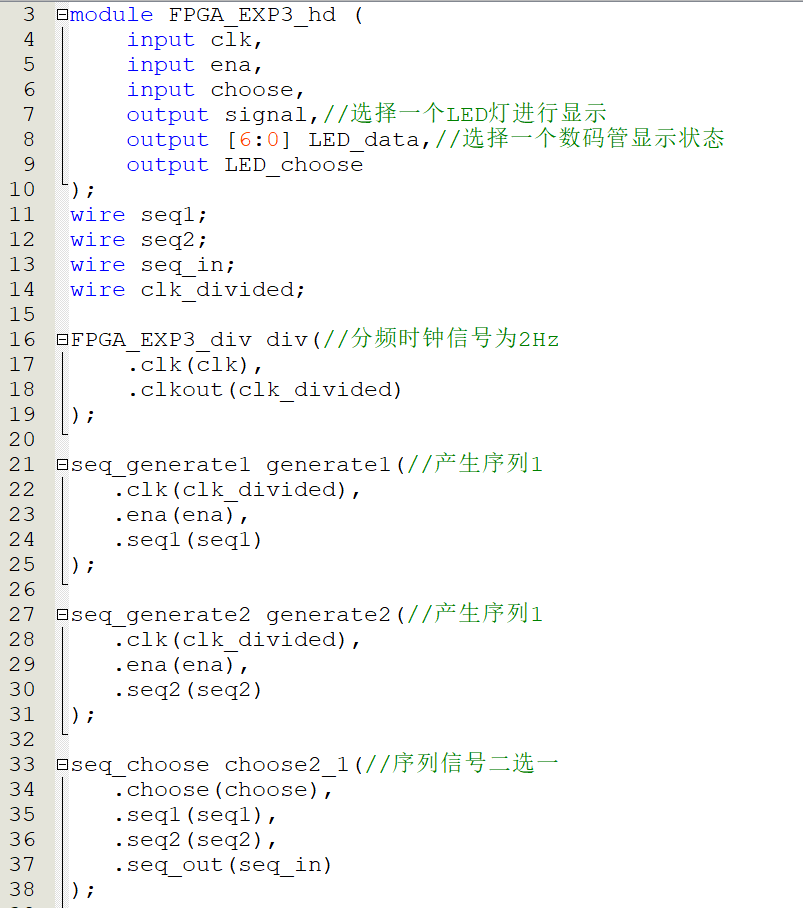
\includegraphics[width=0.5\textwidth]{代码1.png}
    \quad  % 两图之间添加固定间隙（比 \hfill 间距小）
    % 第二张图 
    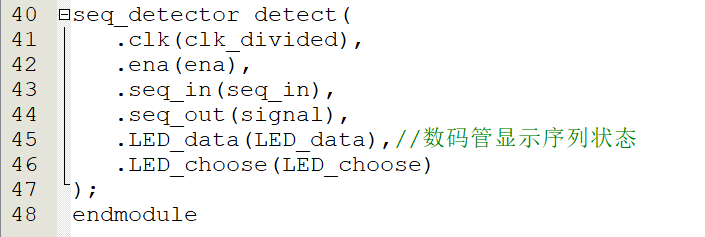
\includegraphics[width=0.5\textwidth]{代码2.png}
\end{figure}
\subsubsection*{3.2 分频模块}
\begin{figure}[ht]
    \centering
    % 第一张图，宽度 0.45 页宽
    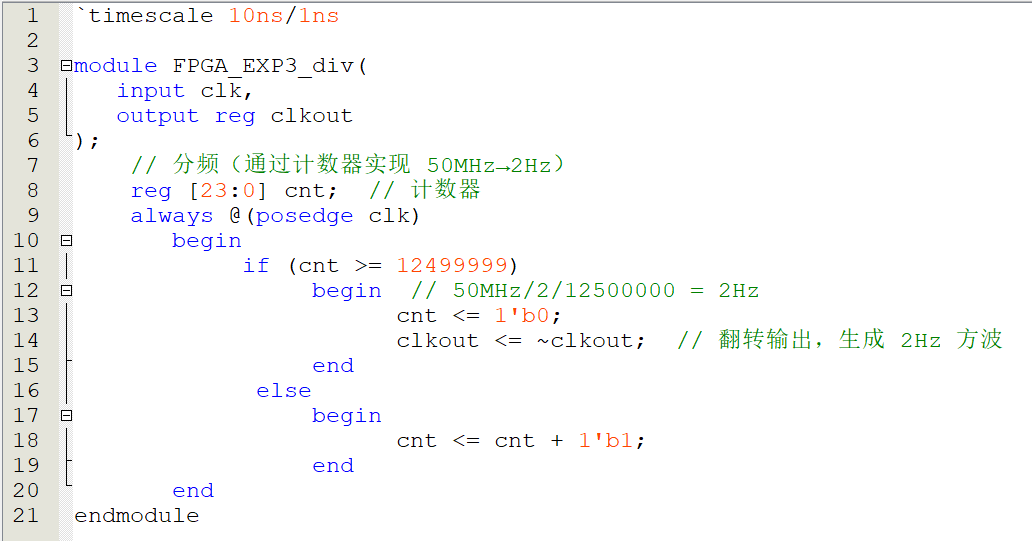
\includegraphics[width=0.55\textwidth]{代码3.png} 
\end{figure}
\subsubsection*{3.3 序列产生模块}
两个序列产生模块代码逻辑基本一致，只是输出的序列不同。所以我只展示其中一个模块的代码。
\begin{figure}[ht]
    \centering
    % 第一张图，宽度 0.45 页宽
    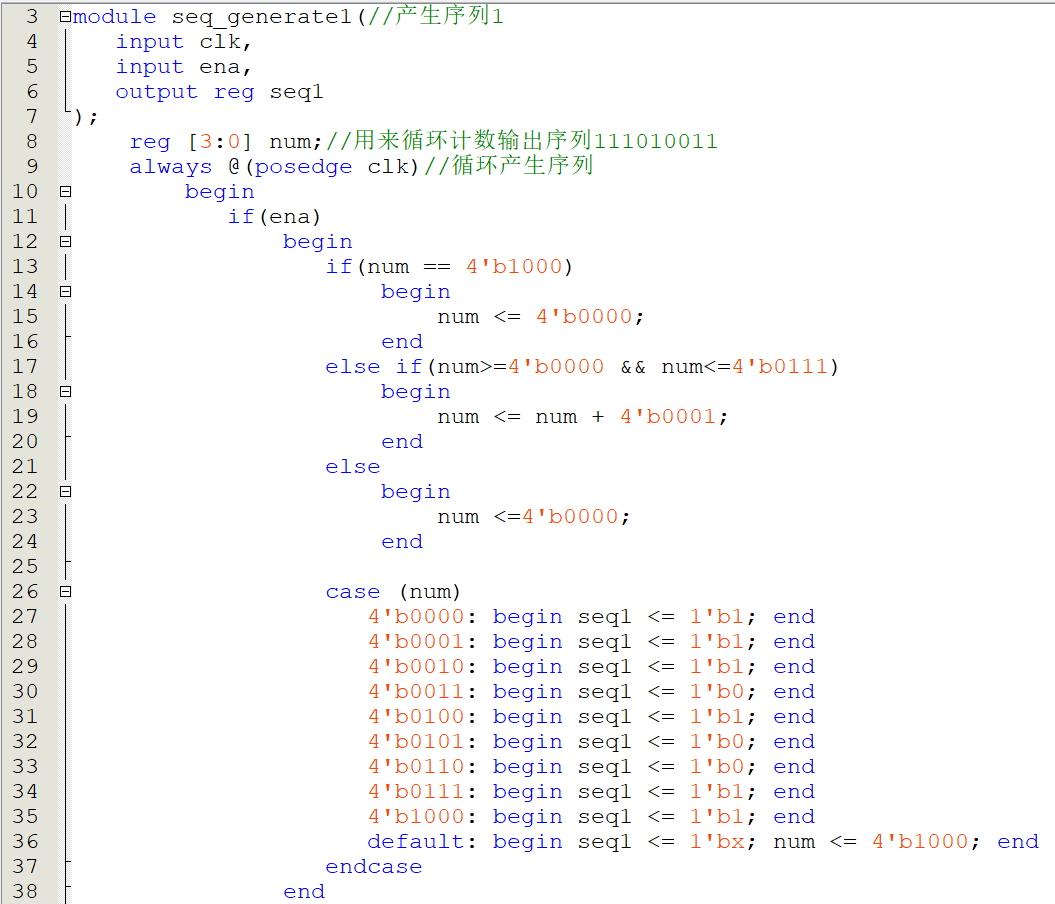
\includegraphics[width=0.6\textwidth]{代码4.png}
    \quad  % 两图之间添加固定间隙（比 \hfill 间距小）
    % 第二张图 
    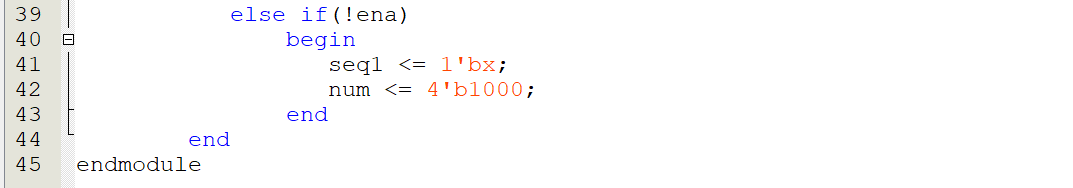
\includegraphics[width=0.6\textwidth]{代码5.png}
\end{figure}
\subsubsection*{3.4 序列选择模块}
\begin{figure}[ht]
    \centering
    % 第一张图，宽度 0.45 页宽
    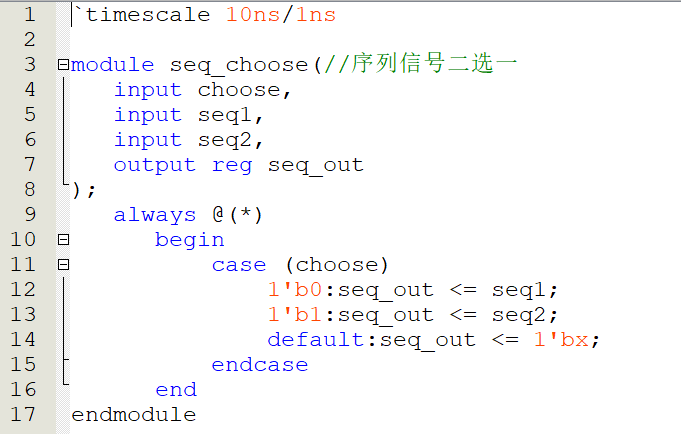
\includegraphics[width=0.6\textwidth]{代码6.png} 
\end{figure}
\subsubsection*{2.5 序列检测模块}
\begin{figure}[ht]
    \centering
    % 第一张图，宽度 0.45 页宽
    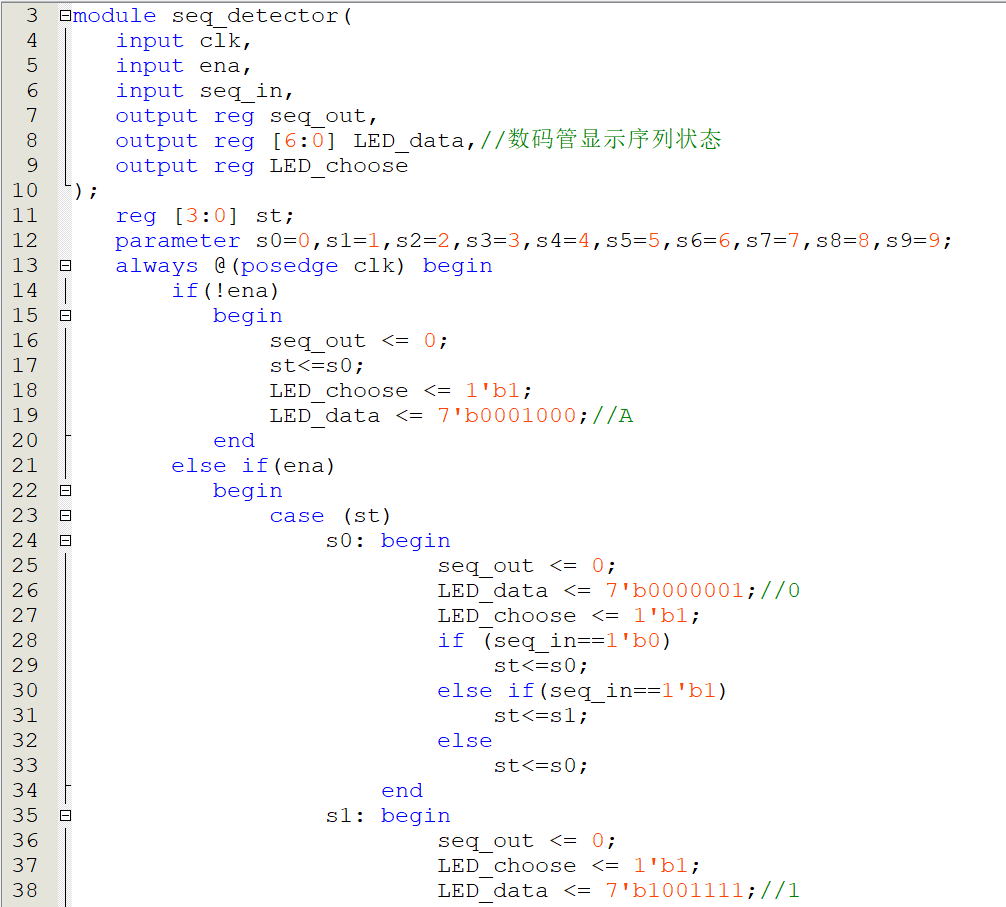
\includegraphics[width=0.56\textwidth]{代码7.png}
    \quad  % 两图之间添加固定间隙（比 \hfill 间距小）
    % 第二张图 
    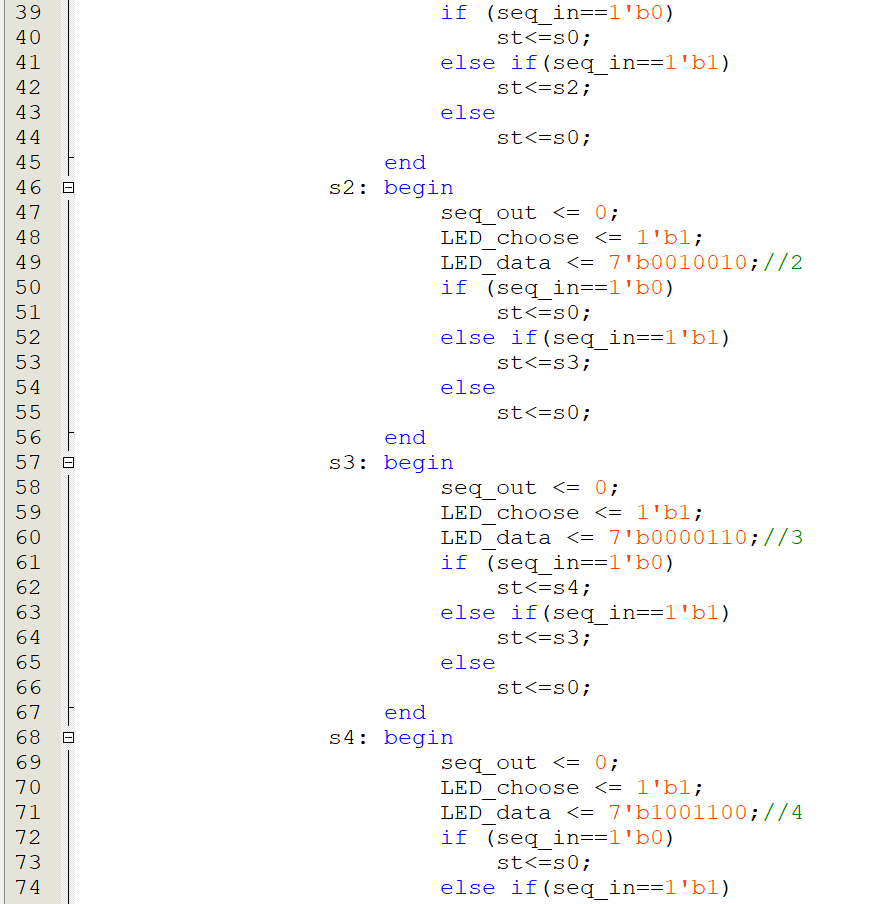
\includegraphics[width=0.56\textwidth]{代码8.png}
\end{figure}

\newpage

\begin{figure}[ht]
    \centering
    % 第一张图，宽度 0.45 页宽
    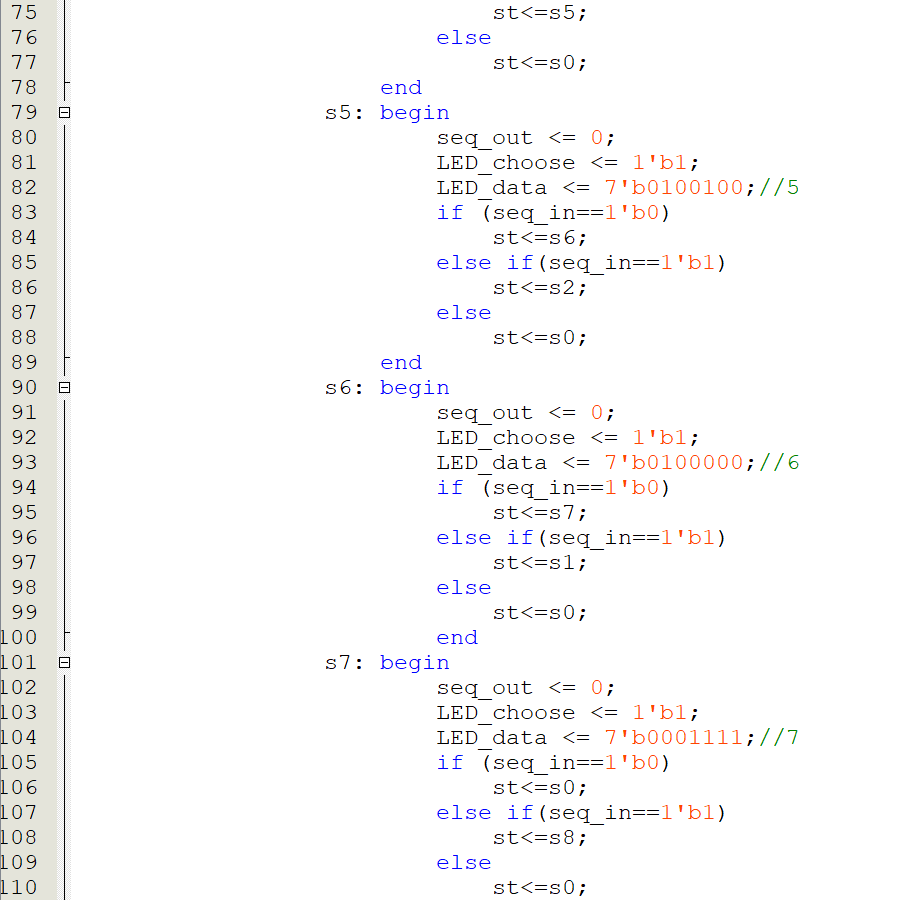
\includegraphics[width=0.55\textwidth]{代码9.png}
    \quad  % 两图之间添加固定间隙（比 \hfill 间距小）
    % 第二张图 
    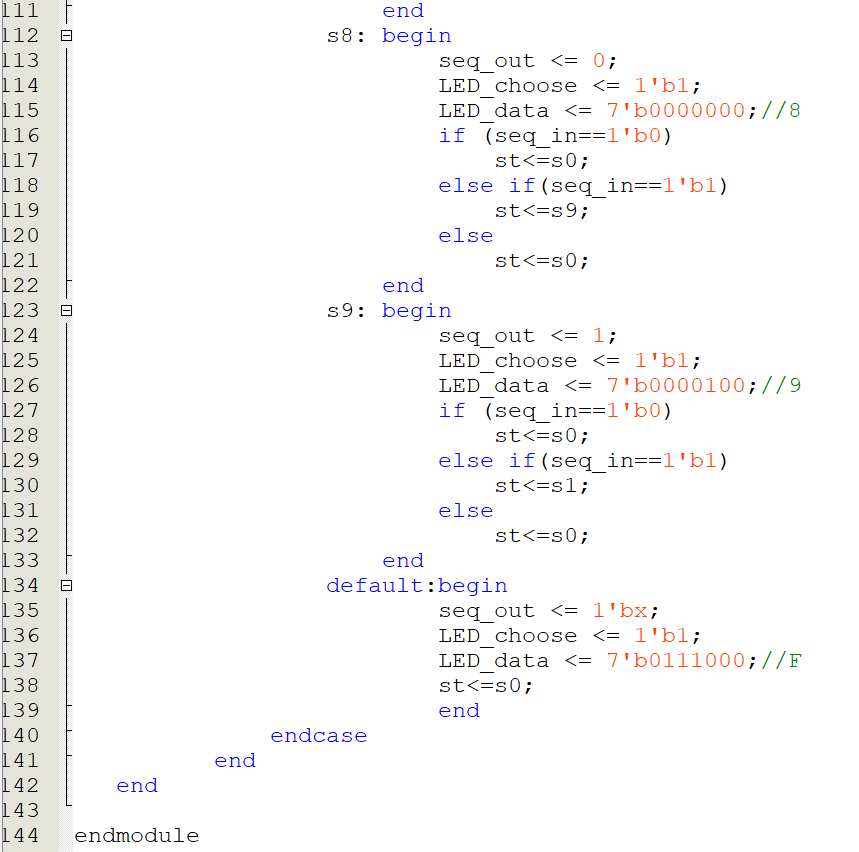
\includegraphics[width=0.55\textwidth]{代码10.png}
\end{figure}

\newpage
\begin{highlightedsection}{}
    四、仿真结果记录
\end{highlightedsection}
\begin{figure}[H]  % H 表示固定图片位置
    \centering
    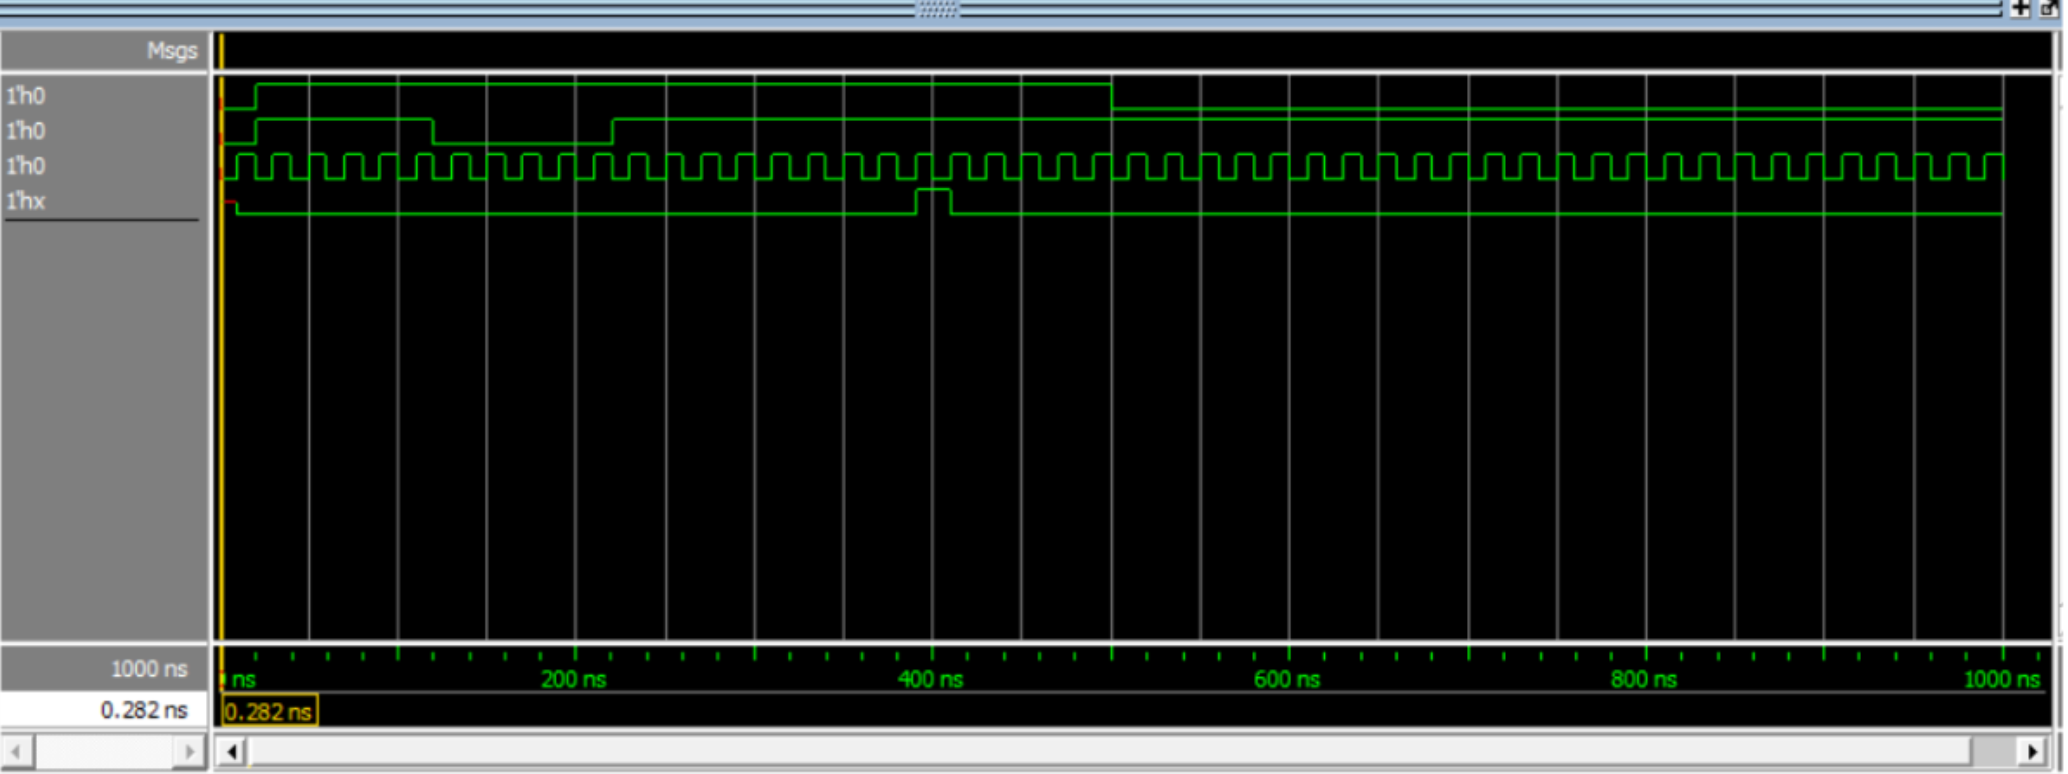
\includegraphics[width=\textwidth]{波形.png}  % 图片的最大宽度为文本宽度
\end{figure}

仿真结果如上图所示，首先choose信号（第一行）置一，选择所需序列，然后使能信号（第二行）置一，模块开始工作，
可以看到初始signal（第四行）输出一直为0，而后使能信号置零，模块停止工作，signal输出保持不变。
经过一段时间后，使能信号再次置一，模块继续工作，signal在经过一段时间后变为1，表明检测到了所需序列。


随后choose信号置零，选择错误序列，然后使能信号置一，模块开始工作，可以看到signal输出一直为0，表明没有检测到所需序列。

仿真结果与预期相符，代码逻辑正确。
\begin{highlightedsection}{}
    五、FPGA验证结果记录
\end{highlightedsection}
我选择DIP0作为使能信号输入，DIP1作为序列选择输入信号(为0输入所需序列，为1输入错误序列)
，一个LED灯用来显示是否检测到
所需序列，一个数码管用来显示当前序列检测器所处状态。

第一次我将DIP1置0，即选择所需序列，然后将DIP0置1，使能整个模块，可以看到数码管循环显示0-9，
并且在数码管显示9的同时LED灯会亮起，表明检测到了所需序列，与理论相符。

随后我将DIP1置1，输出另一个错误的序列，然后将DIP0置1，使能整个模块，
可以看到数码管显示0-4后又显示回了0，这表明检测到的序列不是所需序列，LED灯
也始终没有亮起，与理论相符。

\begin{highlightedsection}{}
    六、实验总结
\end{highlightedsection}
有了实验二的经验，本次实验相对来说轻松了许多，比如说分频模块可以直接借鉴()。

由于老师和助教都推荐把代码分模块编写，本次实验我选择把不同的模块都单独放到不同的文件里，
然后在顶层模块里直接调用相关模块。可以看出整个代码确实清爽了不少，哪个模块有问题也可以单独
修改，便利了不少。

本次实验过程中比较顺利，并未遇到什么问题，希望我后面的代码逻辑能越来越清晰简洁。
\end{document}